\chapter{Paquetes de programación orientados al web scraping}
\label{cha:paquetes de programacion orientados al web scraping}

\section{Búsqueda de paquetes destinados al web scraping}
\label{sec:busqueda de paquetes destinados al web scraping}

Como se especificó en la sección \ref{sec:objetivo y limitaciones} este trabajo se limitará a realizar
una comparativa de los programas software de minado web más frecuentes. Esta comparativa se efectúa con el
fin de conocer cuál o cuáles de estos programas o paquetes software son los más rentables para este propósito.

¿Como saber que paquetes software destinados al minado web son los más comunes? Durante todo este capítulo
se procederá a la búsqueda, selección e introducción de programas software empleados para el web scraping. 
Cabe destacar que Python y R serán los lenguajes de programación con los que se trabajará tanto para el 
desarrollo de la herramienta de comparación, como para el proceso de extracción de datos.

El primer paso consiste en buscar todos los elementos posibles que conforman la población de paquetes
software del mercado, ya sean de Python o R. La búsqueda de estos paquetes se ha realizado a través de las 
distintas fuentes de información mostradas a continuación:

\begin{enumerate}
  \item GitHub \cite{github}. Gran parte de los desarrolladores de estos programas, publican su trabajo en
  estos repositorios de código abierto.
  \item CRAN \cite{cran}. The Comprehensive R Archive Network es una red de servidores ftp y web que
  almacena versiones idénticas de código y documentación para R.
  \item PyPi \cite{pypi}. Python Package Index es un repositorio de software para Python, útil para la
  búsqueda de paquetes de un determinado propósito.
\end{enumerate}

\section{Bibliotecas de Python encontradas durante el proceso de búsqueda}
\label{sec:bibliotecas de python encontradas durante el proceso de busqueda}

A continuación, se hará una breve sinopsis de los paquetes encontrados. Esta introducción tiene como
objetivo conocer el funcionamiento de los paquetes, cuáles son sus funciones y como es el proceso de
extracción. Es posible que algunos de los paquetes hayan sido desarrollados tanto en R como en Python. En 
ese caso, por un lado, la introducción se realzará de forma conjunta, sin embargo, será interesante ver 
el código del mismo en ambos casos y como se comportan estos ante los distintos test de evaluación.

\subsection{Beautiful Soup}
\label{subsec:beautiful soup}

\emph{Beautiful Soup} \cite{beautifulsoup} es una de las librerías de Python más comunes en el ámbito del
web scraping, está diseñada para extraer datos de documentos XML y HTML.

La técnica que emplea este algoritmo consiste en la creación de un árbol de análisis, donde se disponen
todos los elementos del documento como nodos del propio árbol. Una vez disponible, distintos analizadores 
pueden navegar, buscar y modificar este con el fin de obtener la mayor cantidad posible de información.

Beautiful Soup tiene a html.parse como analizador estándar de documentos HTML, pero también admite varios
analizadores de terceros. En la tabla \ref{tab:analizadores disponibles en beautiful soup} se muestran los 
distintos analizadores disponibles, así como un pequeño resumen de las ventajas y desventajas de estos.

\begin{table}[h]
  \begin{center}
  \begin{tabular}{| c | c | c | c |}
  \hline Tipo de analizador & Forma de uso & Ventajas & Desventajas \\ \hline
  html & bs(markup, "html.parser") & Notablemente rapido & Mas lento que lxml\\
  lxml html & 	bs(markup, "lxml") & Muy rapido & Dependencia de C\\
  lxml xml & bs(markup, "xml") & Muy rapido y soporta xml & Dependencia de C\\
  html5lib & bs(markup, "html5lib") & Analiza igual que un buscador & Muy lento\\ \hline
  \end{tabular}
  \caption{Analizadores disponibles en Beautiful Soup}
  \label{tab:analizadores disponibles en beautiful soup}
  \end{center}
\end{table}

El empleo de distintos analizadores supondrá una importancia menor si se aplica sobre documentos bien 
formados, pues la solución aportada presentará la misma estructura que el propio documento original. En 
caso contrario, el uso de diferentes analizadores creará diferentes soluciones para un mismo documento. 
Veamos algún ejemplo.

Se emplea el analizador lxml sobre un documento HTML sencillo pero con erratas. Vemos como la solución 
aportada propone la inclusión de nuevas etiquetas \emph{<head>} y \emph{<body>}, sin embargo, ¿qué ha 
ocurrido con la etiqueta \emph{<p>}?.

\begin{Schunk}
  \begin{Soutput}
    > BeautifulSoup("<a></p>", "lxml")
    # <html><body><a></a></body></html>
  \end{Soutput}
\end{Schunk}

En lugar de ignorar la etiqueta \emph{</p>}, el analizador html5lib la empareja con una etiqueta \emph{<p>}
de apertura. También añade una etiqueta <head> que el analizador lxml habia obviado.

\begin{Schunk}
  \begin{Soutput}
    > BeautifulSoup("<a></p>", "html5lib")
    # <html><head></head><body><a><p></p></a></body></html>
  \end{Soutput}
\end{Schunk}

Al igual que lxml, html.parse ignora la etiqueta de cierre \emph{</p>}. Podemos observar que este analizador 
ni siquiera intenta crear un documento HTML bien formado añadiendo etiquetas \emph{<html>} o \emph{<body>}.

\begin{Schunk}
  \begin{Soutput}
    > BeautifulSoup("<a></p>", "html.parser")
    # <a></a>
  \end{Soutput}
\end{Schunk}

Como vemos diferentes analizadores crearan diferentes soluciones en caso de que el documento a analizar
no este bien formado. Por ello, si deseamos analizar múltiples documentos de los que no conocemos su origen
o estructura sería deseable especificar el tipo de analizador con el fin del obtener la solución deseada.

En cuanto al proceso de extracción que se emplea en este algoritmo es sencillo. En primer lugar, el documento ya sea
HTML o XML se convierte al completo en caracteres Unicode. Tras ello se crea un árbol de objetos donde
cada uno de ellos representa una etiqueta o tag del documento HTML ('<body>, '<p>', ...). Finalmente, un 
analizador especificado por parámetro, recorre el árbol buscando las partes del mismo que se desean.

\begin{figure}[tphb]
  \centering
  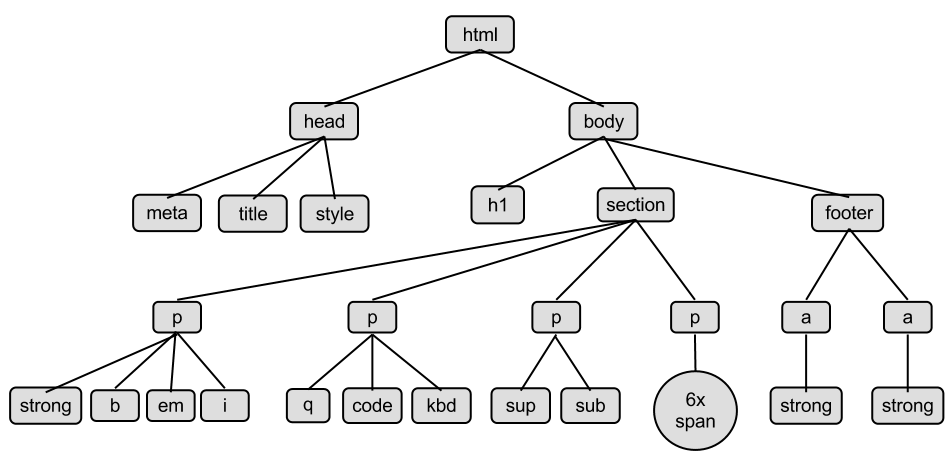
\includegraphics[width=4.5in]{bs-parse-tree.png}
  \caption{Arbol de objetos de Beautiful Soup\cite{bs-parse-tree}}
  \label{img:arbol de objetos de beautiful soup}
\end{figure}

Este algoritmo, no solo permite el recorrido automático del árbol en busca del texto del documento al
completo, sino que permite además la posibilidad de recorrer el mismo de forma manual, por lo que es posible
acceder a todos los objetos del árbol empleando métodos de navegación como \emph{soup.head, soup.parent,
soup.next\_sibling, ...}.

\subsection{JusText}
\label{subsec:justext}

\emph{JusText} \cite{justext} es una herramienta para eliminar el contenido repetitivo, como los enlaces 
de navegación, encabezados y pies de página de las páginas HTML. Está diseñado para preservar principalmente 
el texto que contiene frases completas.

La técnica que emplea este algoritmo consiste en lo que se conoce como segmentación. La idea es formar 
bloques de texto dividiendo la página HTML en etiquetas. Una secuencia de dos o más etiquetas como 
\emph{<br>}, \emph{<div>, ...}, separaría los bloques. 

Aunque no sea habitual, puede ocurrir que el contenido de estos bloques no sea homogéneo, es decir, que 
dentro de un mismo bloque haya una mezcla de información importante con contenido basura. La forma en la 
que JusText separa el contenido basura, denominado boilerplate, del contenido valioso se basa en el volumen 
de palabras con sentido gramatical. Aplicando esta heurística es posible hacer una distinción entre bloques 
como la que sigue:

\begin{itemize}
  \item Los bloques cortos que contienen un enlace son casi siempre del tipo boilerplate.
  \item Los bloques que contienen muchos enlaces son casi siempre del tipo boilerplate.
  \item Los bloques largos que contienen texto gramatical forman parte del contenido valioso, mientras que 
  todos los demás bloques largos son casi siempre del tipo boilerplate.
  \item Tanto los bloques buenos como los bloques de tipo boilerplate tienden a crear grupos, es decir,
  un bloque boilerplate suele estar rodeado de otros bloques de su mismo tipo y viceversa.
\end{itemize}

La dificultad real está en decidir cuando un texto es gramatical y cuando no. Aunque puede ser complicado,
JusText emplea una simple heurística basada en el volumen de palabras con sentido gramatical. Mientras que
un texto gramatical suele contener un cierto porcentaje de este tipo de palabras, como las listas y
enumeraciones, los contenidos de tipo boilerplate suelen carecer de ellas. En definitiva, los bloques
largos y algunos bloques cortos pueden clasificarse con una confianza muy alta. El resto de bloques cortos
pueden clasificarse observando los bloques circundantes.

Con el fin de facilitar el trabajo heurístico, JusText realiza un preprocesamiento del documento HTML. 
Durante esta fase, se elimina el contenido de las etiquetas \emph{<header>}, \emph{<style>} y \emph{<script>}. 
Ademas, el contenido de etiquetas como \emph{<select>} se clasifica inmediatamente como tipo boilerplate. 
Lo mismo ocurre con los bloques que contienen el símbolo de copyright ©.

Tras el proceso de segmentación y preprocesamiento se procede a la clasificación de bloques, donde a cada
uno de estos bloques se le asigna una clase dependiendo de su naturaleza:

\begin{enumerate}
  \item Malo: bloques de tipo boilerplate.
  \item Bueno: bloques pertenecientes al contenido principal.
  \item Corto: bloques demasiado cortos para tomar una decision sobre su naturaleza.
  \item Casi bueno: bloques intermedios entre cortos y buenos.
\end{enumerate}

¿Qué algoritmo sigue JusText para determinar esta clasificación? En el fragmento de código
\ref{cod:justext - algoritmo de clasificacion} se muestra cuál es el proceso de dicha clasificación 
para cada una de los cuatro tipos distintos de bloques. 

\begin{codefloat}
  \inputencoding{latin1}
  \lstinputlisting[style=CppExample]{scripts/clasificacion-justext.py}
  \inputencoding{utf8}
  \caption{JusText - Algoritmo de clasificación}
  \label{cod:justext - algoritmo de clasificacion}
\end{codefloat}

Podemos observar que se definen dos tipos de variables, la densidad y la longitud. Mientras que la longitud 
es el número de caracteres de bloque, la densidad se define como la proporción de caracteres o palabras 
dentro de una una etiqueta de tipo \emph{<a>}, o una lista de parada.

El algoritmo toma como parámetros dos enteros definidos como LENGTH\_LOW(70) y LENGTH\_HIGH(200), ademas 
de tres números de coma flotante, MAX\_LINK\_DENSITY(0.2), STOPWORDS\_LOW(0.3) y STOPWORDS\_HIGH(0.32). 
Los dos primeros establecen los umbrales para dividir los bloques por su longitud en tres tipos, cortos, 
medianos y largos. Los dos últimos dividen los bloques por la densidad de palabras de parada en bajos, 
medianos y altos.

La distinción entre bloques es muy sencilla, hasta ahora JusTest ha sido capaz de clasificar los bloques
buenos y malos, pero ¿qué ocurre con los bloques cortos y los bloques casi buenos? JusText reclasifica
este tipo de bloques en función de los bloques circundantes. Los bloques ya clasificados como buenos o
malos sirven como piedras base en esta etapa y su clasificación se considera fiable, por lo que nunca se
modifica. Esta reclasificación se puede ver resumida en la imagen \ref{img:justext - reclasificacion de
bloques}.

\begin{figure}[tphb]
  \centering
  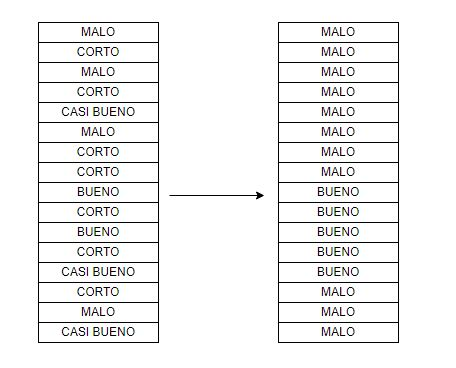
\includegraphics[width=4in]{justext-blocks-classification.jpg}
  \caption{JusText - Reclasificación de bloques}
  \label{img:justext - reclasificacion de bloques}
\end{figure}

La idea que subyace a la reclasificación es que los bloques 'boilerplate' suelen estar rodeados de otros 
bloques 'boilerplate' y viceversa. Los bloques casi buenos suelen contener datos útiles del corpus si se 
encuentran cerca de bloques buenos. Los bloques cortos suelen ser útiles sólo si están rodeados de bloques 
buenos por ambos lados.

\subsection{Inscriptis}
\label{subsec:inscriptis}

\emph{Inscriptis} \cite{inscriptis} es una biblioteca de conversión de HTML a texto basada en Python. Esta
librería es especialmente adecuada para aplicaciones que requieran representaciones de texto con una alta
precisión y calidad del contenido HTML.

A diferencia de otros algoritmos de extracción Inscriptis no solo tiene en cuenta el texto extraído, sino
que además la estructura del mismo es muy importante, por lo que este texto extraído podría acercarse más 
al obtenido por cualquier navegador web. 

Veamos una pequeña comparación entre la extracción de texto de Beautiful Soup \ref{subsec:beautiful soup}, 
con la extracción de texto de Inscriptis, donde se tiene un fragmento HTML como el siguiente, como objeto 
de prueba.

\begin{Schunk}
  \begin{Soutput}
    <ul>
        <li>first</li>
        <li>second</li>
    <ul>
  \end{Soutput}
\end{Schunk}

Si aplicásemos Beautiful Soup sobre este fragmento HTML el texto extraído sería algo como \emph{'firstsecond'},
donde no se tiene en cuenta el diseño ni la estructura del documento. Sin embargo, si aplicamos Inscriptis
sobre el mismo fragmento HTML, la salida obtenida sería la siguiente:

\begin{Schunk}
  \begin{Soutput}
    * first
    * second
  \end{Soutput}
\end{Schunk}

Inscriptis, no solo admite construcciones tan simples como la anterior, permite analizar construcciones 
mucho más complejas, como las tablas anidadas, y subconjuntos de atributos HTML y CSS donde es esencial 
una conversión precisa de HTML a texto.

La técnica que emplea Inscriptis se conoce como reglas de anotación, es decir, mapeos que permiten anotar 
el texto extraído. Estas anotaciones se basan en la información estructural y semántica codificada en las 
etiquetas y atributos HTML utilizados para controlar la estructura y diseño del documento original. 

Con el fin de asignar etiquetas y/o atributos HTML a las anotaciones, se emplea un algo parecido a un 
diccionario. En el diccionario mostrado a continuación, la etiqueta \emph{<h1>} produce las anotaciones 
heading y h1, una etiqueta \emph{<div>} con una clase que contiene el valor toc da como resultado la 
anotación table-of-contents, y todas las etiquetas con un atributo cite se anotan con citation.

\begin{Schunk}
  \begin{Soutput}
    {
      "h1": ["heading", "h1"],
      "h2": ["heading", "h2"],
      "b": ["emphasis"],
      "div#class=toc": ["table-of-contents"],
      "#class=FactBox": ["fact-box"],
      "#cite": ["citation"]
    }
  \end{Soutput}
\end{Schunk}

Imaginemos que se dispone de un documento HTML como el que sigue y unas reglas de anotación determinadas.

\begin{Schunk}
  \begin{Soutput}
    <h1>Chur</h1>
    <b>Chur</b> is the capital and largest town of the Swiss canton of the Grisons 
    and lies in the Grisonian Rhine Valley.
  \end{Soutput}
\end{Schunk}

En este ejemplo, la salida habitual según el diccionario anterior debería ser una etiqueta de cabecera y
otra de énfasis, veamos la salida que proporciona el proceso de asignación.

\begin{Schunk}
  \begin{Soutput}
    {"text": "Chur\n\nChur is the capital and largest town of the Swiss canton
          of the Grisons and lies in the Grisonian Rhine Valley.",
    "label": [[0, 4, "heading"], [0, 4, "h1"], [6, 10, "emphasis"]]}
  \end{Soutput}
\end{Schunk}

Como era de esperar la obtención del texto es precisa, pero no solo del texto sino de su estructura. Además,
la asignación de etiquetas también se ha realizado de forma correcta.

\subsection{Goose3}
\label{subsec:goose3}

\emph{Goose} \cite{goose3} es una librería de programación cuyo objetivo es la extracción de texto en 
artículos. Inicialmente, el proyecto fue iniciado con Java, pero han surgido nuevas versiones en diferentes 
lenguajes de programación como Scala o Python.

El objetivo del software es tomar cualquier artículo de noticias o página web de tipo artículo y no solo
extraer lo que es el cuerpo principal, sino también se extraen todos los metadatos e imágenes del mismo.
Goose extraerá: (1) texto principal del artículo, (2) imagen principal del artículo, (3) videos introducidos
en el artículo, (4) descripción y (5) meta tags.

La técnica que emplea Goose3 para la extracción de texto es muy similar a la que se emplea en Beautiful Soup
\ref{subsec:beautiful soup}, donde un árbol se recorre con el fin de obtener la mayor cantidad de información
valiosa posible.

\begin{codefloat}
  \inputencoding{latin1}
  \lstinputlisting[style=CppExample]{scripts/extraccion-goose3.py}
  \inputencoding{utf8}
  \caption{Goose3 - Algoritmo de extracción}
  \label{cod:goose3 - algoritmo de extraccion}
\end{codefloat}

Si observamos el algoritmo \ref{cod:goose3 - algoritmo de extraccion}, si se determina que en un cierto
nodo del árbol contiene texto, se crea un nuevo nodo y este se inserta en una lista. Con este proceso
todos los nodos que contienen información valiosa son agrupados y almacenados para su posterior uso.

Al igual que con Beautiful Soup, Goose puede emplear distintos analizadores, html de lxml o el conocido como
soup parser de lxml. Pero no solo es posible configurar el analizador, también se puede determinar el agente
de usuario que se empleará para la extracción.

\begin{Schunk}
  \begin{Soutput}
    > g = Goose({'browser_user_agent': 'Mozilla', 'parser_class':'soup'})
  \end{Soutput}
\end{Schunk}

\subsection{News-please}
\label{subsec:news-please}

\emph{News-please} \cite{news-please} es un web scraper y web crawler de código abierto escrito en Python
desarrollado para cumplir cinco requisitos: (1) extracción de noticias de cualquier sitio web, (2) extracción
completa del sitio web, (3) alta calidad de la información extraída, (4) facilidad de uso y (5) mantenibilidad.

A diferencia de otros web scrapers ya mencionados anteriormente, news-please emplea herramientas ya existentes,
las cuales se amplían con nuevas funcionalidades con el objetivo de cumplir con los requisitos señalados.

\begin{figure}[tphb]
  \centering
  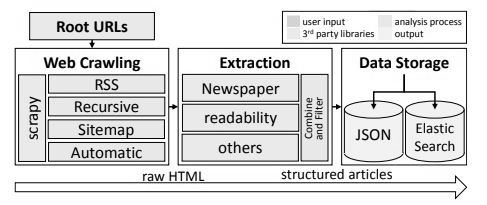
\includegraphics[width=4.5in]{newsplease-processing.jpg}
  \caption{News-please - Proceso de scraping y crawling}
  \label{img:news-please - proceso de scraping y crawling}
\end{figure}

En cuanto al proceso de web crawling, news-please lo divide en dos subtareas, en primer lugar se descarga 
el documento HTML empleando el framework \emph{Scrapy}. En segundo lugar, con el objetivo de encontrar 
todos los artículos publicados en dicho documento se admiten cuatro técnicas:

\begin{enumerate}
  \item RSS \footnote{formato XML para distribuir contenido en la web}: análisis de los canales RSS para 
  encontrar los artículos recientes.
  \item Recursiva: seguimiento de los enlaces enlaces internos en las páginas rastreadas.
  \item Sitemap \footnote{Un sitemap es un archivo que enumera las URL visibles de un determinado sitio, 
  el objetivo principal es revelar dónde pueden buscar contenido las máquinas.}: analiza los sitemaps en 
  busca de enlaces a todos los artículos.
  \item Automático: prueba los sitemaps, vuelve a ser recursivo en caso de error.
\end{enumerate}

Estos cuatro enfoques también pueden combinarse, por ejemplo, iniciando dos instancias de news-please en 
paralelo, una en modo automático para obtener todos los artículos publicados hasta el momento y otra 
instancia en modo RSS para recuperar los artículos recientes.

Para el proceso de web scraping, se emplean herramientas ya existentes en el mercado con el objetivo de 
obtener la información deseada, es decir, título, párrafo principal, contenido principal, autor, fecha e 
imagen principal. Por un lado, news-please ha decidido utilizar herramientas como \emph{Newspaper} 
\ref{subsec:news-paper} o \emph{Readability} \ref{subsec:readability} para el proceso de extracción del 
contenido principal en artículos, mientras que por otro se emplea \emph{Regex} para la extracción de fechas 
de publicación.

\subsection{Trafilatura}
\label{subsec:trafilatura}

\emph{Trafilatura} \cite{trafilatura} es un paquete de Python que descarga, analiza y extrae datos de páginas
web. Combina dos bibliotecas de web scraping ya existentes, \emph{Readability} \ref{subsec:readability} y
\emph{JusText} \ref{subsec:justext} como redes de seguridad y fallbacks.

La técnica que emplea el algoritmo de extracción de este paquete se fundamenta en una cascada de filtros
basados en reglas y heurística de contenido. Veremos que al igual que muchos otros algoritmos de extracción,
usa los árboles de objetos como estructura de datos.

En primer lugar, se realiza lo que se conoce como delimitaciones de contenido, donde mediante expresiones
XPath dirigidas y atributos HTML comunes, se excluyen partes no deseadas del código HTML creando un árbol
de objetos. Las mismas operaciones se realizan para los comentarios en caso de que formen parte de la
extracción.

\begin{codefloat}
  \inputencoding{latin1}
  \lstinputlisting[style=CppExample]{scripts/delimitacion-trafilatura.py}
  \inputencoding{utf8}
  \caption{Trafilatura - Delimitación de contenido}
  \label{cod:trafilatura - delimitacion de contenido}
\end{codefloat}

Si se detecta que la extracción realizada ha sido posiblemente defectuosa, se ejecuta lo que se conocen 
como algoritmos de respaldo. Estos aplican una heurística basada en la longitud de las líneas, la relación 
texto/marcado y la posición/profundidad de los elementos en el árbol HTML. Una vez aplicados estos 
algoritmos, su resultado se compara con la extracción 'casera' y se determina la extracción más eficaz, 
sobre todo en términos de longitud e impurezas.

Por último, es caso de que ambas soluciones provoquen una salida defectuosa, se ejecuta una extracción base
con el fin de buscar elementos de texto 'salvajes' que probablemente se hayan pasado por alto. Esto implica
la búsqueda de cualquier elemento con contenido textual útil.

\begin{codefloat}
  \inputencoding{latin1}
  \lstinputlisting[style=CppExample]{scripts/respaldo-trafilatura.py}
  \inputencoding{utf8}
  \caption{Trafilatura - Algoritmo de respaldo y extraccion base}
  \label{cod:trafilatura - algoritmo de respaldo}
\end{codefloat}

Como resultado de toda esta consecucion de algoritmos se obtienen los textos principales y los posibles 
comentarios de los documento HTML analizados, con la posibilidad de conservar elementos estructurales como
párrafos, títulos, listas, comillas, código, saltos de línea, formato de texto en línea... En la extraccion, 
también se incluyen metadatos, es decir, título, nombre del sitio, autor, fecha, categorías y etiquetas.

\subsection{Dragnet}
\label{subsec:dragnet}

\emph{Dragnet} \cite{dragnet} es un web scraper escrito en Python y construido sobre el entorno de cálculo
numérico 'numpy/scipy/Cython'. Como hemos visto hasta ahora, el objetivo de cualquier algoritmo de
extracción es separar el contenido principal del contenido de navegación, los bloques de publicidad, los
avisos de copyright y similares en las páginas web. La mayoría de estos algoritmos emplean heurísticas
determinas para este fin. Dragnet se encarga de realizar esta separación de contenido empleando el
aprendizaje automático.

El algoritmo comienza dividiendo el documento HTML en una secuencia de bloques utilizando el DOM 
\footnote{El DOM define la manera en que objetos y elementos se relacionan entre sí en el navegador y en 
el documento. \cite{dom-wikipedia}} y un conjunto específico de etiquetas como \emph{<div>}, \emph{<p>} o
\emph{<h1>}, que modifican la estructura del propio documento. Iterando por el DOM, cada vez que el algoritmo 
se encuentra alguna de las etiquetas mencionadas anteriormente, se crea un nuevo bloque. Aquellos bloques
sin contenido de valor, son descartados. 

Una vez separado el documento en bloques, se deben asignar un conjunto de características a cada uno. Estas 
serán útiles en un clasificador con el objetivo de predecir el contenido con valor, del contenido 
'boilerplate' a nivel de bloque. Cualquier bloque con más del 10\% de los tokens extraídos se etiqueta 
como contenido valioso.

La primera característica consiste en la densidad de texto y enlaces. La intuición es que los bloques de 
contenido tienen una mayor densidad de texto y una menor densidad de enlaces que los bloques denominados 
boilerplate, ya que muchos de estos ultimos son bloques que consisten en breves fragmentos de palabras o 
son principalmente texto ancla. 

El segundo tipo de característica está diseñada heurísticamente para capturar información semántica en el
código HTML que dejan los programadores. Muchos atributos como \emph{id} o \emph{class}, y etiquetas HTML 
incluían tokens tipo \emph{comment}, \emph{header} y \emph{nav}. Estos nombres descriptivos son utilizados 
por los programadores cuando escriben CSS y Javascript y, puesto que se eligen con el objetivo de que tengan 
sentido para el programador, incorporan cierta información semántica sobre el contenido del bloque.

\begin{table}[h]
  \begin{center}
  \begin{tabular}{| c | c | c | c |}
  \hline Token & Content : No Content & Percent of blocks  \\ \hline
  menu & 1 : 372.6 & 2.2\% \\
  widget & 1 : 314.1 & 4.6\% \\
  nav & 1 : 68.9 & 3.3\% \\
  facebook & 1 : 18.3 & 1.3\% \\
  top & 1 : 13.3 & 1.9\% \\
  twitter & 1 : 8.5 & 2.3\% \\
  title & 1 : 3.3 & 10.5\% \\
  header & 1 : 2.9 & 3.7\% \\ \hline
  comment & 3.2 : 1 & 21.3\% \\
  author & 4.9 : 1 & 7.9\% \\
  thread & 5.0 : 1 & 3.0\% \\
  avatar & 42.1 : 1 & 3.2\% \\ \hline
  \end{tabular}
  \caption{Comparación de tokens en el atributo \emph{class}}
  \label{tab:Comparacion de tokens en el atributo class}
  \end{center}
\end{table}

En la tabla \ref{tab:Comparacion de tokens en el atributo class} se enumeran algunos tokens seleccionados
en el atributo de clase junto con sus ratios de probabilidad de contenido y no contenido. Los tokens de la
parte superior de la tabla tienen más probabilidades de aparecer en bloques sin contenido, mientras que los
de la parte inferior tienen más probabilidades de aparecer en bloques con contenido. Para una mejor 
visualización, se forman dos grupos, según estén asociados a bloques de no contenido o de contenido.

Finalmente, la tercera característica incluye varias ideas. Por un lado, la relación entre la longitud del 
texto y el número de etiquetas HTML tiende a ser mayor en los bloques de contenido. En segundo lugar, las 
secciones de la página que no son de contenido tienden a estar agrupadas, de modo que la diferencia en la 
proporción de contenido y etiquetas de un bloque a otro tiende a ser pequeña en las regiones que no son de 
contenido. La idea final es combinar la proporción de etiquetas de contenido y la diferencia en la 
proporción de etiquetas de contenido en un enfoque de agrupación de k-means no supervisado, de modo que 
los bloques sin contenido se agrupen naturalmente cerca del origen.

\subsection{Readability}
\label{subsec:readability}

\subsection{HTML-Text}
\label{subsec:html-text}

\emph{HTML-Text} \cite{html-text} es una librería software destinada a la extracción de texto en documentos
HTML. Las principales diferencias entre emplear expresiones XPath \emph{.xpath('//text()')} o emplear
otros algoritmo de extracción como Beautiful Soup \emph{.get\_text()} son: (1) Por un lado, el texto extraído
es limpio, ya que no contiene estilos en línea, javascript o comentarios los normalmente no son visibles 
para los usuarios, (2) en segundo lugar, se normalizan los espacios en blanco de una forma más inteligente 
que empleando \emph{.xpath('normalize-space())}, (3) por último, se añaden nuevas líneas para que el texto 
de salida se parezca más a cómo se representa en los navegadores. 

\subsection{Newspaper3k}
\label{subsec:news-paper}

\section{Paquetes de R encontrados durante el proceso de búsqueda}
\label{sec:paquetes de r encontrados durante el proceso de busqueda}

\section{Paquetes seleccionados para el proceso de análisis}
\label{sec:paquetes seleccionados para el proceso de analisis}
